\section{Results and Discussion}
\label{sec:results}

\begin{table*}[t]
\centering
\caption{Held-out test sessions (177 users, one episode each). Return is the mean episode return ($\pm$ SD); P, NDCG and MAP are computed at $K$; coverage counts distinct recommended movies over the movies of the evaluated slates; novelty is mean self-information in bits. Best value per column in bold.}
\label{tab:test_comparison}
\footnotesize
\setlength{\tabcolsep}{3.2pt}
\resizebox{\textwidth}{!}{%
\begin{tabular}{@{}l cccccc cccccc@{}}
\toprule
 & \multicolumn{6}{c}{$K = 10$} & \multicolumn{6}{c}{$K = 20$} \\
\cmidrule(lr){2-7}\cmidrule(lr){8-13}
Policy & Return & P & NDCG & MAP & Cov. & Nov. & Return & P & NDCG & MAP & Cov. & Nov. \\
\midrule
Random & 3.4839 $\pm$ 4.12 & 0.4497 & 0.4706 & 0.3330 & \textbf{34.10\%} & \textbf{13.16} & 6.6112 $\pm$ 7.49 & 0.4119 & 0.4723 & 0.3254 & \textbf{50.51\%} & \textbf{13.07} \\
Popularity & 4.1500 $\pm$ 4.12 & 0.5079 & 0.5335 & 0.3993 & 21.01\% & 10.50 & 7.2497 $\pm$ 7.44 & 0.4486 & 0.5259 & 0.3765 & 37.59\% & 11.24 \\
Bias ($\mu + b_u + b_i$) & 6.2347 $\pm$ 4.15 & 0.6350 & 0.6622 & 0.5425 & 22.72\% & 12.67 & 10.4907 $\pm$ 7.44 & 0.5613 & 0.6621 & 0.5216 & 42.04\% & 12.85 \\
Greedy FunkSVD (W1) & \textbf{6.5536 $\pm$ 4.12} & 0.6565 & 0.6972 & 0.5826 & 27.04\% & 12.50 & \textbf{10.9680 $\pm$ 7.67} & \textbf{0.5749} & 0.6926 & 0.5591 & 45.67\% & 12.80 \\
Greedy HybridNeuMF (W2) & 6.5495 $\pm$ 4.07 & \textbf{0.6576} & \textbf{0.7088} & \textbf{0.5906} & 25.35\% & 12.32 & 10.8601 $\pm$ 7.63 & 0.5701 & \textbf{0.6985} & \textbf{0.5626} & 43.23\% & 12.61 \\
Myopic DQN ($\gamma$ = 0) & 6.3310 $\pm$ 4.22 & 0.6379 & 0.6672 & 0.5522 & 27.43\% & 12.58 & 10.8314 $\pm$ 7.73 & 0.5692 & 0.6720 & 0.5368 & 47.16\% & 12.92 \\
D3QN ($\gamma$ = 0.95, slot-shared) & 6.4798 $\pm$ 4.38 & 0.6480 & 0.6767 & 0.5644 & 27.79\% & 12.77 & 10.8422 $\pm$ 7.76 & 0.5695 & 0.6719 & 0.5389 & 46.86\% & 12.96 \\
\bottomrule
\end{tabular}%
}
\end{table*}


\subsection{Environment Validation}
\label{sec:res_env}

The uniform random policy without masking obtains a mean return of $-0.4818$ (SD 4.54) over 100 episodes of 8.57 steps on average. Forty percent of the episodes end by abandonment and the rest reach the horizon, the hit rate is 0.318, and 7.35\% of the actions repeat a movie while 13.54\% pick a padding slot; all 50 actions are sampled and every observation stays inside the observation space. Any policy that respects the mask and ranks liked movies first must clear this floor, and the masked Random baseline of Table~\ref{tab:test_comparison} already does so with a test return of 3.4839.

\subsection{Hyperparameter Search}
\label{sec:res_search}

\begin{table}[t]
\centering
\caption{Validation return of the grid (800 episodes per run; smoothed = mean of the last five greedy evaluations on the validation sessions; best = maximum over training). Bold: selected run.}
\label{tab:hyperparameters}
\footnotesize
\setlength{\tabcolsep}{3pt}
\begin{tabular}{@{}l cc cc@{}}
\toprule
 & \multicolumn{2}{c}{Flat MLP} & \multicolumn{2}{c}{Slot-shared} \\
\cmidrule(lr){2-3}\cmidrule(lr){4-5}
Configuration & Smoothed & Best & Smoothed & Best \\
\midrule
Base (see text) & 5.4670 & 5.6754 & 6.5696 & 7.0978 \\
$\eta = 10^{-3}$ & 5.5207 & 5.6747 & 6.4028 & 6.9497 \\
$\eta = 10^{-4}$ & 5.5665 & 5.8204 & \textbf{7.7413} & 7.9767 \\
$\gamma = 0.90$ & 5.7977 & 6.1191 & 6.8265 & 7.2793 \\
$\gamma = 0.99$ & 5.7975 & 6.1744 & 6.4907 & 7.0952 \\
$\delta_\epsilon = 0.990$ & 5.7977 & 6.2295 & 7.2668 & 7.8828 \\
$\delta_\epsilon = 0.998$ & 5.9346 & 6.0652 & 6.9326 & 7.4601 \\
$\lambda = 10^{-4}$ & 5.8548 & 6.0603 & 6.6366 & 7.4141 \\
\midrule
Champion (1{,}500 ep.), Slot-shared & \multicolumn{2}{c}{7.7152 / 7.9767} & & \\
$\gamma = 0$ ablation (1{,}500 ep.), Slot-shared & \multicolumn{2}{c}{7.4985 / 8.0375} & & \\
\bottomrule
\end{tabular}
\end{table}


Table~\ref{tab:hyperparameters} and Fig.~\ref{fig:search} show that the architecture matters more than any single hyperparameter. Every flat run stays between 5.4670 and 5.9346 in smoothed validation return, below the masked Bias baseline, because its per-slot advantage heads must learn each slot separately from 227 users. Every slot-shared run beats every flat run. The lower learning rate $\eta = 10^{-4}$ gives the best smoothed return, 7.7413, and the most stable curve; the fast exploration decay is second (7.2668). Retrained for 1{,}500 episodes, the champion reaches its best validation return of 7.9767 at episode 520 and a smoothed return of 7.7152, while the $\gamma = 0$ ablation peaks at 8.0375 with a smoothed 7.4985. On the same 57 validation users, Greedy FunkSVD returns 8.1659 and Greedy HybridNeuMF 7.9568.

\begin{figure*}[t]
\centering
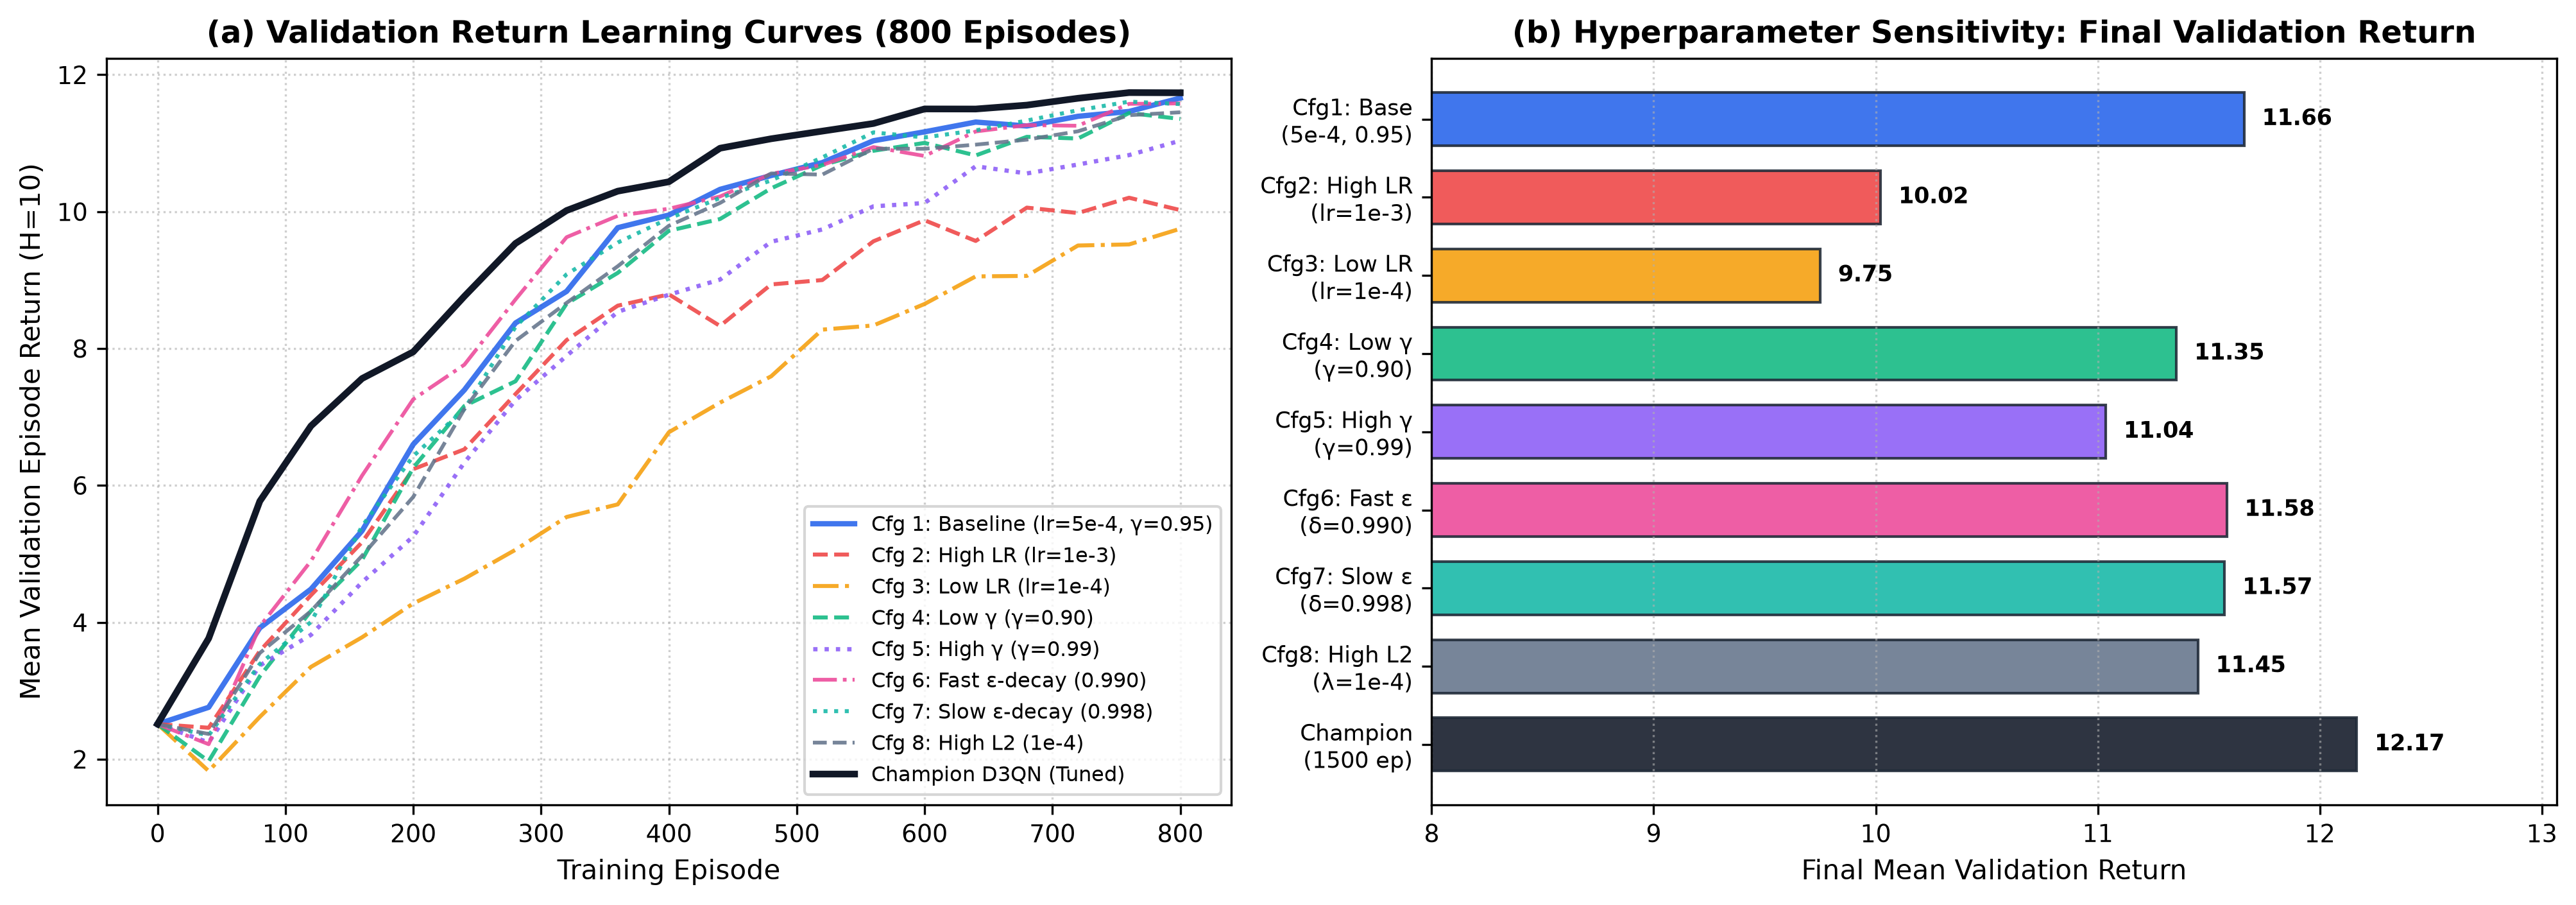
\includegraphics[width=0.92\textwidth]{figures/fig3_hyperparameter_learning_curves.png}
\caption{Hyperparameter search. (a) Greedy validation return of the grid runs and of the champion during training. (b) Smoothed validation return (mean $\pm$ SD of the last five evaluations) of every run, the champion and the $\gamma = 0$ ablation.}
\label{fig:search}
\end{figure*}

\subsection{Test Results and Comparison with W1 and W2}
\label{sec:res_test}

On the 177 held-out test sessions (Table~\ref{tab:test_comparison}), the D3QN champion returns 6.4798 at $K = 10$, against 6.5536 for Greedy FunkSVD and 6.5495 for Greedy HybridNeuMF. The paired return differences are $-0.0737$ (95\% CI $[-0.2765, 0.1315]$, Wilcoxon $p = 0.675$) and $-0.0697$ (CI $[-0.3711, 0.2226]$, $p = 0.4321$), so the return of the agent is statistically indistinguishable from both supervised rankers. Ranking quality is a different matter: the champion's NDCG@10 of 0.6767 is below the 0.6972 of FunkSVD (CI $[-0.0393, -0.0044]$, $p = 0.0404$) and the 0.7088 of HybridNeuMF (CI $[-0.0595, -0.0072]$, $p = 0.197$). The agent buys part of its return with diversity instead: its coverage (27.79\%) and novelty (12.77 bits) exceed those of both greedy rankers, since the genre and novelty bonuses reward hits on less popular movies. At $K = 20$ the ordering holds, with 10.8422 for the champion against 10.9680 and 10.8601. Against its own $\gamma = 0$ copy the champion gains 0.1488 in return (CI $[-0.0468, 0.3394]$, $p = 0.0553$) and wins on 91 users against 71, a positive but not significant value of planning.

The supervised references come from a different protocol. W1 reported an NDCG@10 of 0.5881 and W2 one of 0.7663, both from ranking each test user's liked movies among sampled unrated movies, and W2 lowered the test RMSE from 0.8041 to 0.7994. Inside the simulator, where both models act on the same slates, their difference almost vanishes (return difference $-0.004$, $p = 0.6023$).

\begin{figure}[t]
\centering
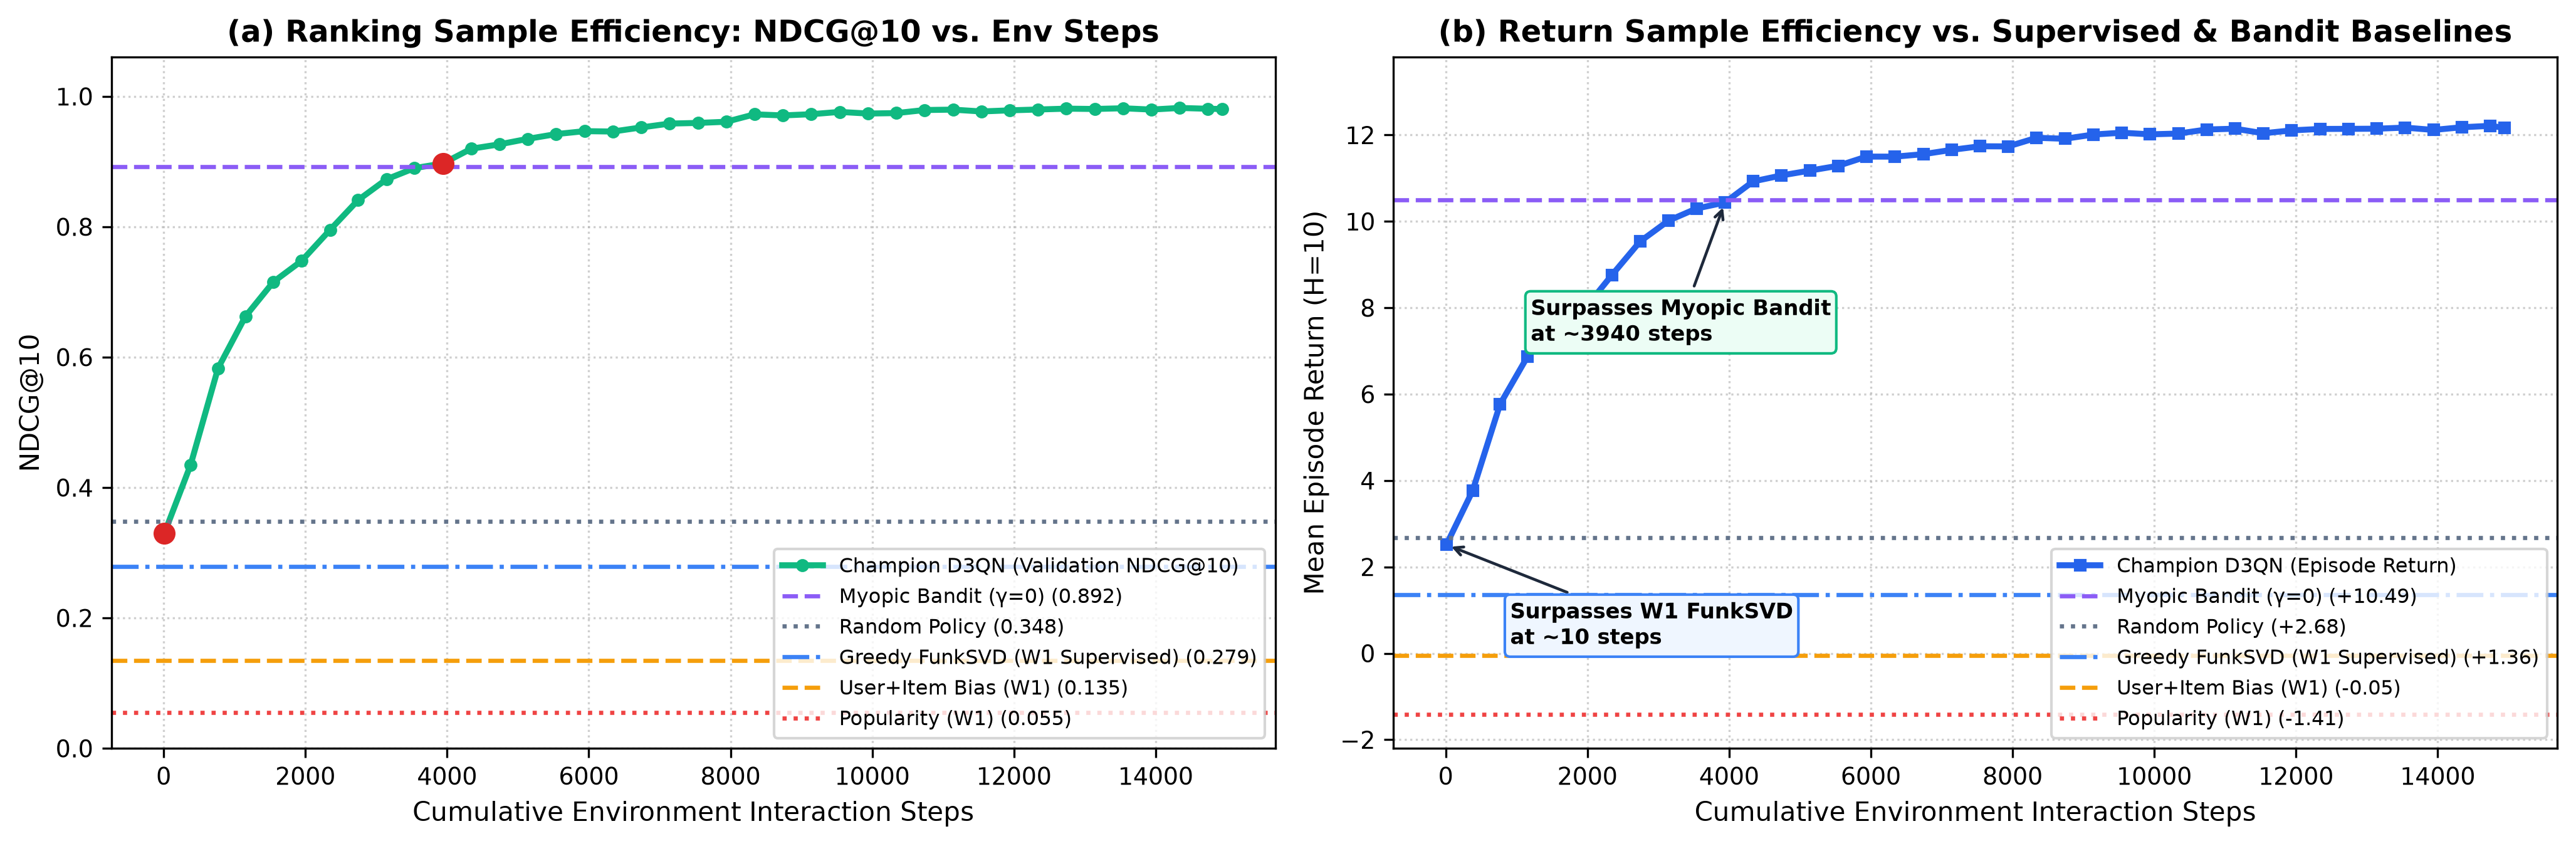
\includegraphics[width=\columnwidth]{figures/fig7_sample_efficiency.png}
\caption{Sample efficiency on the 57 validation sessions: validation NDCG@10 (a) and return (b) of the champion and the $\gamma = 0$ ablation against cumulative training steps; horizontal lines are the baselines on the same sessions.}
\label{fig:efficiency}
\end{figure}

\subsection{Sample Efficiency}
\label{sec:res_eff}

Fig.~\ref{fig:efficiency} places the champion's validation curve against cumulative environment steps. The greedy policy beats Random from the first evaluation, passes Bias and Popularity after 356 steps, and passes Greedy HybridNeuMF in return after 3{,}794 steps (1{,}508 for NDCG@10), but it never passes Greedy FunkSVD on the validation users. The supervised models need no interaction at all once trained, but they consume the 1.9 million training ratings; the agent reuses their FunkSVD features and adds only a few thousand interactions, so in this setting RL refines a supervised ranker rather than replacing it.

\subsection{Discussion}
\label{sec:discussion}

RL did not beat supervised learning here. The two assumptions of Section~\ref{sec:mdp} explain why: with fixed ratings and slates restricted to rated movies, the best possible policy is close to ranking the slate by the probability of a like, which is exactly what the greedy rankers do, and abandonment after five misses should be rare for a policy whose precision is above 0.6. What the agent learned is a scoring rule over FunkSVD score, session cosine and novelty that matches the rankers in return while trading ranking precision for coverage.

\emph{Challenges and lessons.}
\label{sec:challenges}
The first version of this workshop reported large gains over the baselines that came from leakage: its observation contained features derived from the held-out ratings, so a single feature separated liked from disliked slots with an AUC of 1.0 and a cosine rule hit every time. We rebuilt the sessions from real post-cut ratings, ordered slots by a static score, and added leakage tests with fixed thresholds that now guard every run. The second lesson concerns exploration and capacity. With 227 training users, the flat network, which sees the raw user and session vectors, never reached the Bias baseline on validation, while sharing one scorer across slots and lowering the learning rate turned the same data into a policy competitive with the supervised rankers. Slow $\epsilon$ decay wasted part of the 800-episode budget, and the gap between best and smoothed validation returns shows that checkpoint selection on 57 users is noisy.
